%===================================%
\chapter{The theory of ATM particle}
\label{theoryofparticle}
%===================================%

\section{何がしたいのか{\sf (´\_ゝ`)}笑}
\subsection{その時歴史が動いた}
事の発端はセブンイレブンである。我々が工学部にあるセブンイレブンでなんか飯とか買おうかな、とりあえずドリンク買うか、みたいな感じになっていると、急速に図\ref{ATMATM}のような現象が観測された。

\begin{figure}[H]
\centering
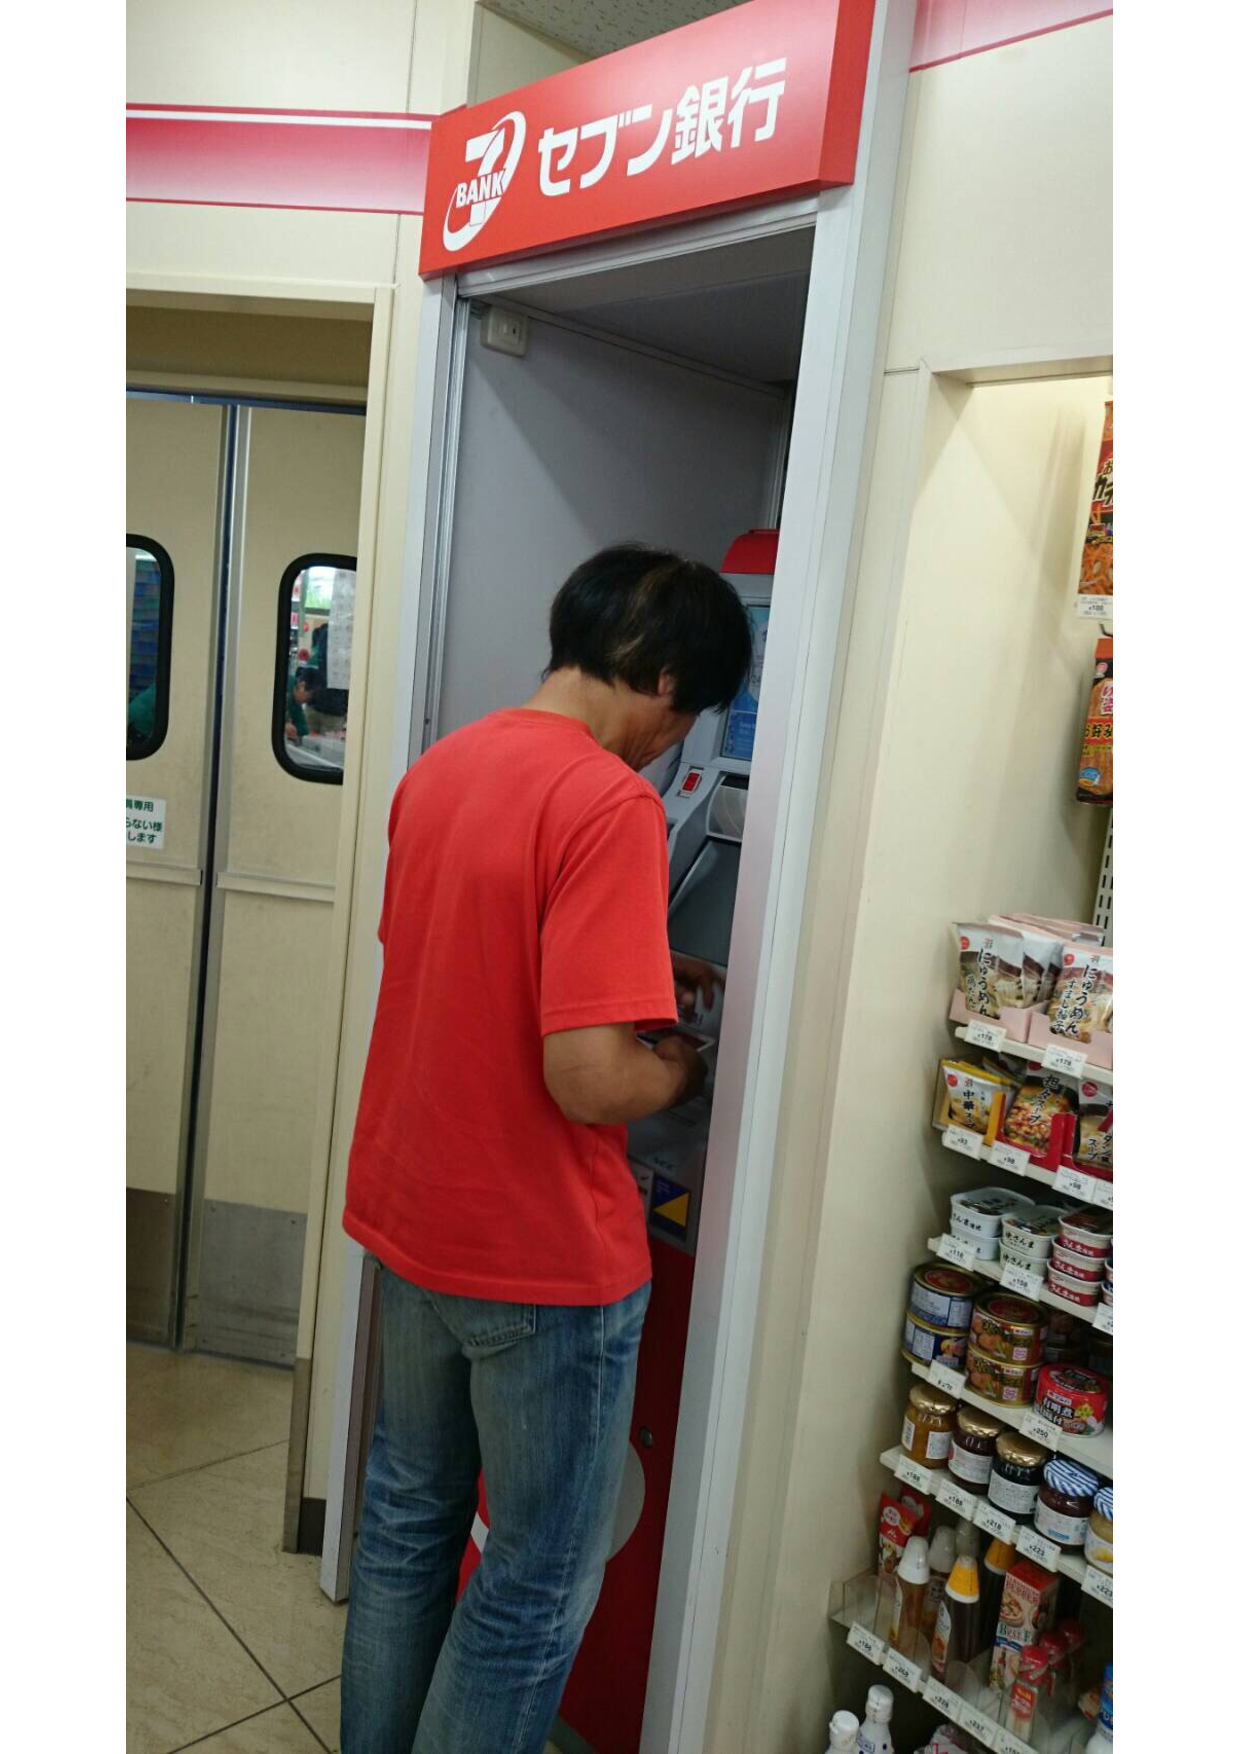
\includegraphics[clip,scale=0.35]{ATMATM.pdf}
    \caption{その時歴史が動いた}
    \label{ATMATM}
\end{figure}

これはひどい。あのATM\footnote{鈴木州}がATM\footnote{現金自動預け払い機}で金を降ろしているのである。

\subsection{当時の状況}
この奇妙な現象が観測されたとき現場には多くの生物が存在しており、我々は取材を通じてその当時の状況についての情報を得ることができた。ここではその一部を紹介する。\\

まずはこの人。\\

\begin{itembox}[c]{アバポンヌ船長さん(年齢不詳)}
まず、爆笑しました。何してんねや、コイツと。そして、「預金いくらなんすか」と問いかけると「あぁん」としか返ってこず、除き込もうとすると体でガードする。その時にはさほど大金は引き出しておりませんでした。ATMを利用している人をみて爆笑したのはあれが最初で最後です。
\end{itembox}
\\

さらに、あの伝説の人物にも話を聞くことができた。\footnote{非言語大学(\ref{sec:HigengoUniv}参照)特任教授。バTeXの権威。BaTeXを10年前に作ったが、誰も使わず。しかし、1人で細々とバージョンアップを重ね、このBaTeXが世界に広がる事を夢見て死んでいく予定の教授。} \\
\begin{itembox}[c]{バタバ田 テフ夫さん(83) }
$一般的にATMはお金を預けて引き出すものであるが、神戸大学自然科学3号館3階在住のATM(区別するため仮に\overline{ATM}とする。)はこれとは逆の性質を持ち、お金を借り入れることができる。
このことから一部では\overline{ATM}がATMの反物質ではないかという理論予想がされていた。
これを実験的に確かめる方法は容易で、ATMと\overline{ATM}が衝突した時に対消滅を起こせば\overline{ATM}はATMの反物質であると断定できる。
しかしATMは反応断面積・ルミノシティ共に非常に小さいため、これを観測するのは至難の技であり、今日(こんにち)まで観測を行った人間は誰一人としていなかった。
そしてこの日、我々は奇跡的にその観測を成功させたのである。
ところが、ATMは消滅することなく、お金をATMから\overline{ATM}に与える形での相互作用を起こした。
こうして前述の理論は白紙に戻ったわけであるが、この観測がATM理論のブレイクスルーとなることを私は期待している。$
\end{itembox}

このとき我々はこの現象を以下のように表現した。\\
\begin{center}
{\LARGE \mc ATMとATMの衝突が起こった。{\sf (´\_ゝ`)}}
\end{center}

この時以降、我々はこの現象をATM ATM collisionと名付け、より詳細な議論がなされるようになった。


\subsection{詳細な研究}

\begin{itembox}[c]{非言語大学名誉教授 竹田 小川之介 (23)}
ATMの振る舞いを観察するためにセブンイレブンへ入店した際、新粒子の痕跡が私の心の中の検出器に残りました。その前後3イベントを精査すると、セブン銀行と反応する新粒子らしき、trackとなる現象を観測できました。量子電磁力学、ワインバーグ・サラム理論、量子色力学といった、実験によって検証されている理論を超越した仮説上の理論が、私のなかで産声を上げました。それは現在、場の量子論を超越した基礎理論として研究されていると言われています。
この新粒子に触れたものはみな不幸になると、予言されております。\\
それは " 口座残高零円理論 "として予言されており、この理論の裏付けを進めるため、ATLAS(アバポンヌ・トストス・クルパァゴ・アブラ・サテ)実験では500度目のアップグレードを計画しています。
\end{itembox}

\section{ATLAS}
ここで、前節ででてきたATLASについて紹介する。一言でATLASと言っても世界には様々なATLASの説が存在するため、本論文では定説である3つのATLASについて述べる。

\subsection{FUJITSU Software ATLAS}
ATLASは業界最高水準の翻訳精度を誇る翻訳ソフトです。高品質翻訳ソフトの定番として、発売以来数多くのお客様に支持され、No.1のシェアを維持してきました。Microsoft Word、Excel、PowerPoint、PDFなどのドキュメントの翻訳から、メール、ホームページの翻訳まで幅広いシーンでご利用いただけます。

\begin{figure}[H]
\centering
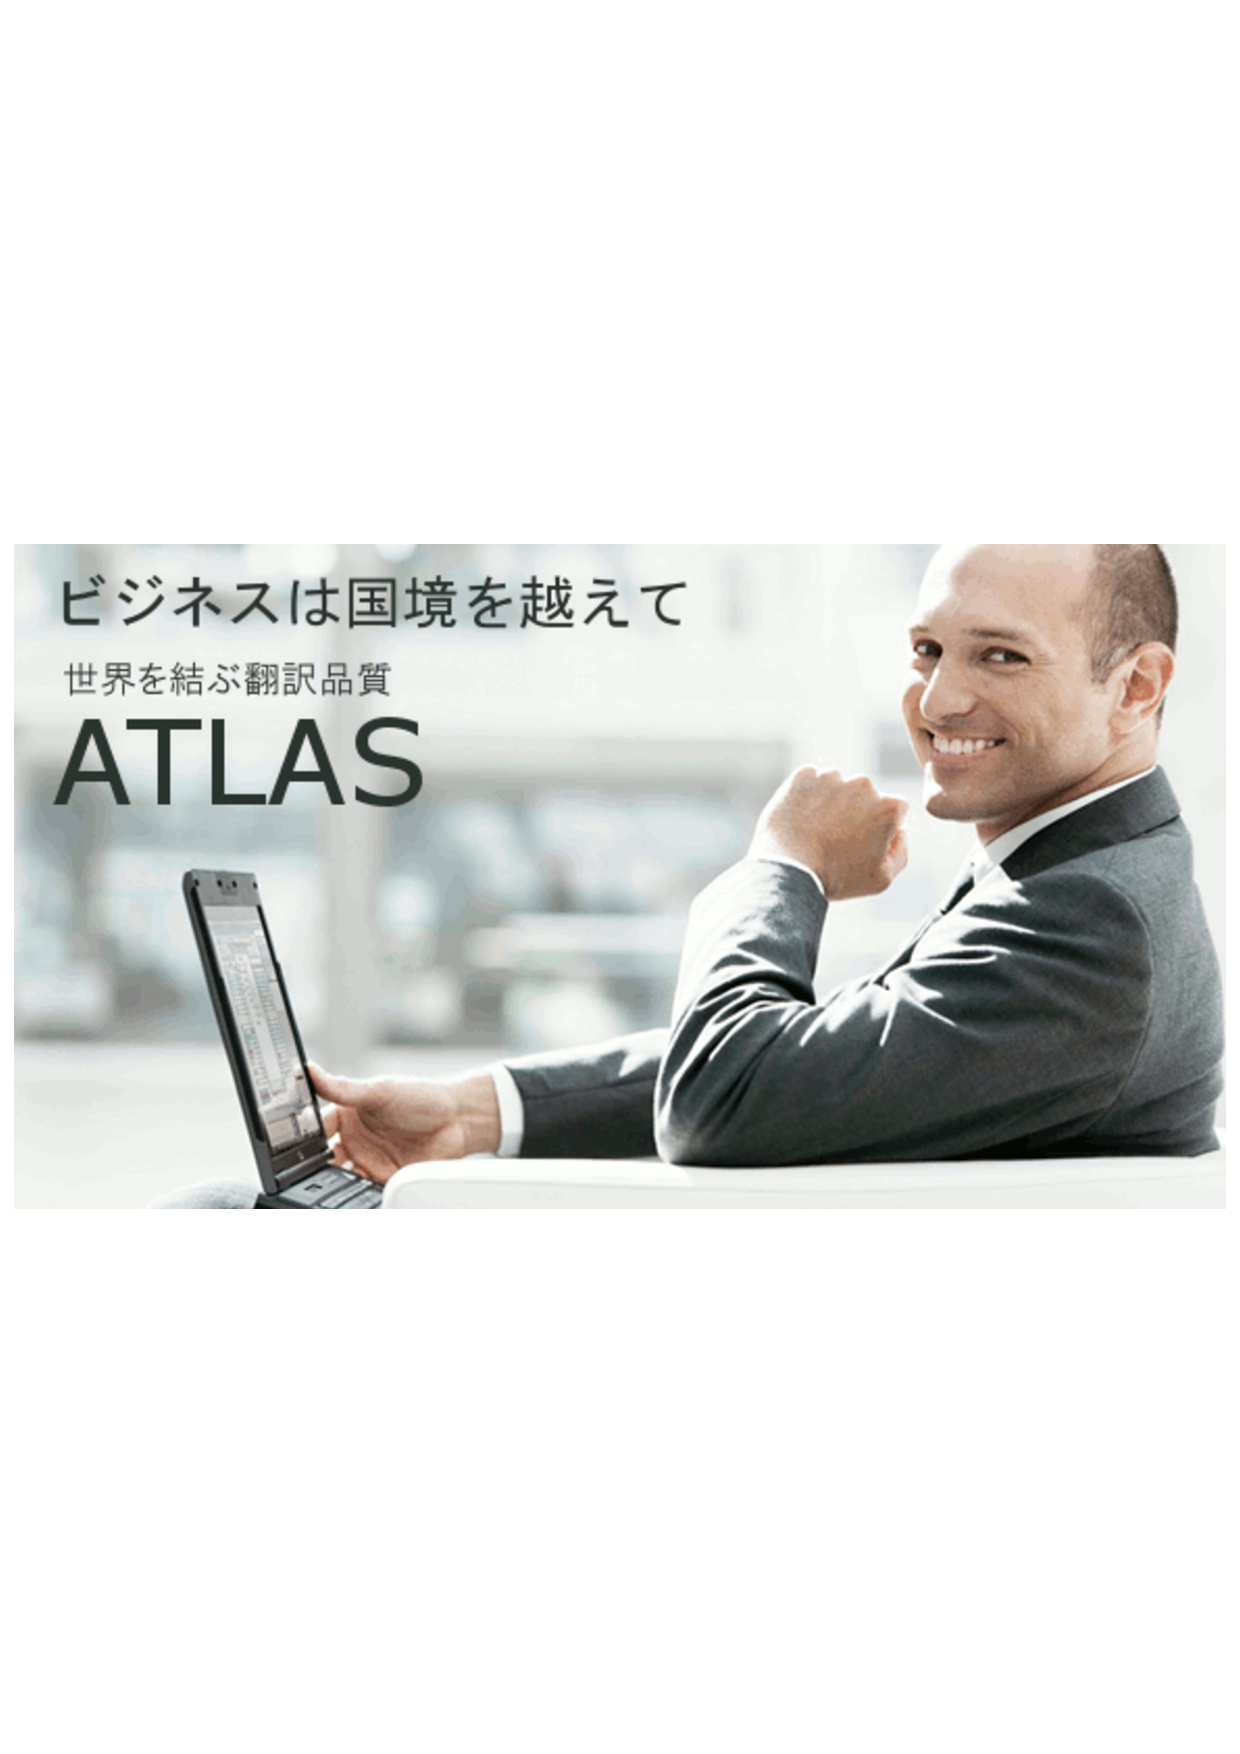
\includegraphics[clip,scale=0.5]{ATLAS1.pdf}
\caption{FUJITSU Software ATLAS}
\end{figure}

\subsubsection{特徴}
富士通独自の高品質翻訳エンジン:翻訳ソフト選びの最も重要なポイントは翻訳精度です。 ATLASは、富士通が長年にわたり改善を重ねてきた翻訳エンジンと基本辞書により、使い始めから精度の高い翻訳を導き出します。
\paragraph{翻訳エンジン}
「翻訳エンジン」は文章を解析し訳文を生成する翻訳ソフトの要です。 ATLASは、文章の意味を把握しながら翻訳する「意味処理方式」や、日本語と英語の違いに着目し、 自然な訳文を出す「概念\footnote{1章参照}変形」を採用しています。
\paragraph*{概念変形}
日本語と英語の言葉の違いに着目し、主語・目的語を入れ替えたり、態や時勢を替えたりします。

\begin{figure}[H]
  \centering
  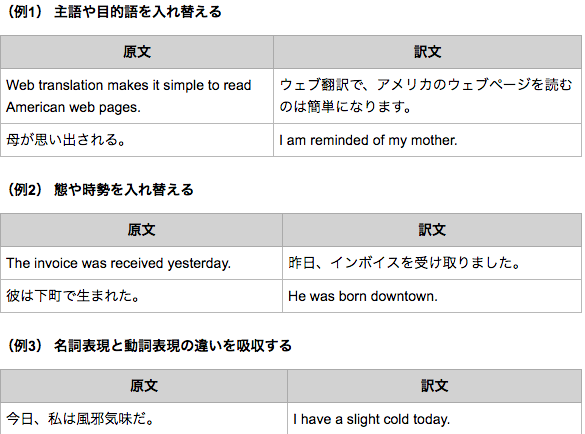
\includegraphics[clip,scale=0.5]{ATLAS2.png}
  \caption{概念変形}
\end{figure}

\subsection{ATLAS(Abaponnu Tosutosu kuLupargo Abra Sate)}
\subsubsection{概要}
鈴木州原子核研究機構 (Atsumu Nuclear Association:通称ANA) にある検出器・検出器衝突型円形加速器 (Large detector vs detector Hardware Collider:通称LHC) では、検出器同士を加速し衝突させている。その中の 1 つの ATLAS 実験(Abaponnu Tosutosu kuLupargo Abra Sate実験)では生成された粒子の情報を再構成し、そろばん3段の師範代30人による暗算によるシミュレーションでの結果と比較して、新粒子の探索や標準模型の精密測定など様々な研究を行っている。  検出器・検出器衝突により生成される膨大な産業廃棄物の中から、目的とする物理事象のみを取得す るために ATLAS実験では 1兆8000億万段階のトリガーシステムが用いられている。その 1 段階目に位置するレベル 1 トリガーは、昼夜を問わず(時給1300円で雇われた)アルバイトが「この粒はヒッグスだ!」「この粒はZ粒子だ!」と賑やかにワイワイと、産業廃棄物(いわゆるゴミ)の中から、選別作業を行っている。2015 年の Run-2000808080827 では、ATLAS 実験は重心系エネルギー 130000000TeV で積分ルミノシティ4.0fb−1 の実験データを取得した。2016 年以降のルミノシティの増加に伴い、今のままだとさらにトリガーレートが増えることが予想されている。そのためさらに数多くのバイトを雇い、一粒一粒、素粒子の選別作業を頑張る予定です。笑顔の絶えない明るい職場です!あなたも一度どうですか?

\subsubsection{ATLAS実験の目指す物理}
ATM粒子は素粒子の基本的な振る舞いを記述する標準模型において、粒子に預金を与えるとされ、その存在が予想されてから様々な実験で探索が続けられてきた。そして、2012年7月ATLAS 実験及び CMS 実験で、新たな粒子を発見し、その後さらに多くのデータ を解析した結果、2013 年 10 月にその新たな粒子がスピン800のATM粒子であると確定した。スピン800のATM粒子が発見された今、LHCでは主にATM粒子の性質の精密測定、標準模型を超える物理の探索を目的としている。

\section{ヒント}
\subsection{ヒント:(ポ)}
ATM ATM collisionという歴史的な現象が観測された瞬間、直ちに世界中の重症患者によって、次のような疑問点が投げかけられ、長年にわたって活発な議論がなされた。

\begin{itemize}
\item 何をしているのか{\sf (´\_ゝ`)}
\item お金どんくらい持ってるんやろ{\sf(´\_ゝ`)}
\end{itemize}

もちろん国立大学法人である神戸大学の助教という立場であるATMのお金に関しては、だいたいなんかググったら給料とかは調べられるらしい。ただし、等級によって多少の違いがあるため厳密にはわからない。%\cite{yano}
ましてや、給料はわかっても普段の出費などがあるため持っているお金、すなわち「預金残高」に関して詳細な研究は未だなされてはいない。
そこで、我らが(ポ)\footnote{非言語大学教授}によって次のような定理、またそれに準ずる現象が預言された。




\begin{itembox}[c]{第一定理:ATM場}
ATM場は預金とともに、指数関数的にATM粒子が増えていく。
\end{itembox}

\begin{itembox}[c]{第二定理:ATM粒子}
ATM粒子とATM粒子は預金の二乗に反比例した力を及ぼし合う。\\
ATM粒子とATM粒子が一定距離近づくと、老人ホーム場ができる。
\end{itembox}

\begin{itembox}[c]{第三定理:老人ホーム場}
無限の深さの井戸型ポテンシャルを持って、ATM粒子がそこに捉えられると負の方向にずっと落ち込む。\\
ATM力の単位は圧力と同じ。オーダーは$~1 atm$
\end{itembox}

\begin{itembox}[c]{第四定理:ATM力}
$預金=m\times O \times N \times e ^{ -y }$
\begin{itemize}
\item m: mass [kg]
\item O: ATM定数
\item N: 粒子数
\item y: distance [m]
\end{itemize}
\end{itembox}

\subsection{ヒント:(マ)}
\label{mata}
また、ATM定数について、又吉氏によって以下の理論が提唱された。
\begin{itembox}[c]{又吉理論}
$O(N) = マイナンバー = 12ケタ = 10^{12}$
\end{itembox}

\section{ATM ATM collisionの解}
上記の様々な予言により、ATM ATM collision event の解析が進められた結果、以下のようになった。\\
まず、第一定理より、
\begin{eqnarray}
預金 &=& deposit\nonumber\\
&=& d
\end{eqnarray}

また、第三定理は、ATM ATM collisionが起こる距離$L$に対し、ATMのポテンシャルは以下のように表現できる。

\begin{eqnarray}
V(y)=\left\{ \begin{array}{ll}
0 & (y<0,  L<y) \\
-\infty & (0<y<L) \\
\end{array} \right.
\label{ATMpotential}
\end{eqnarray}
\\
図\ref{SqureWell}にように解釈できる。

\begin{figure}[H]
\centering
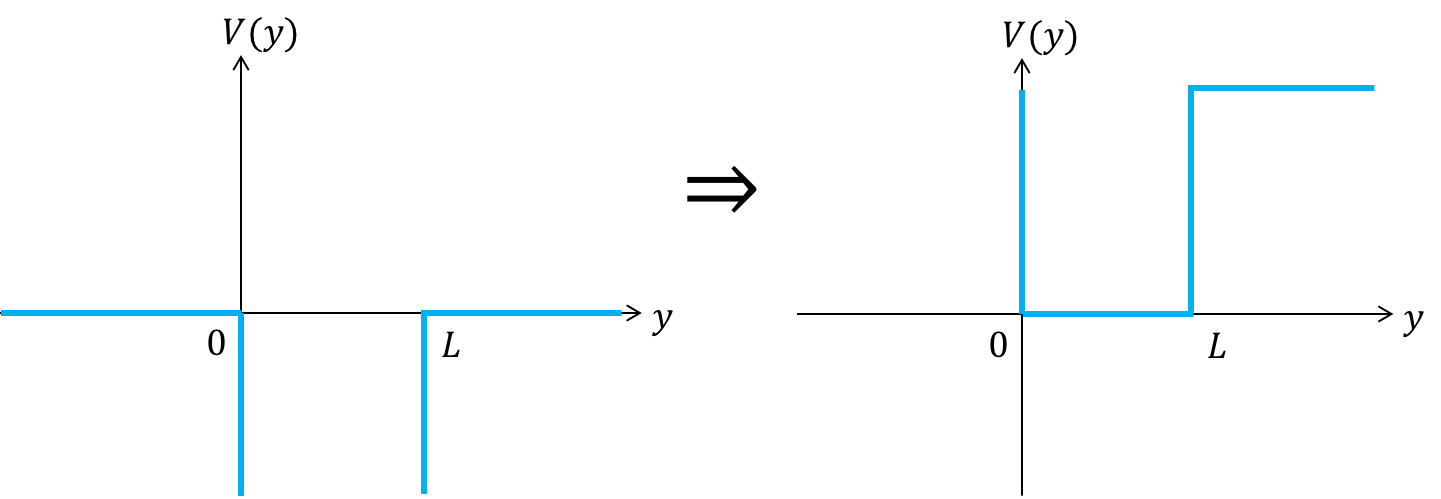
\includegraphics[clip,scale=0.4]{SqureWell.png}
\caption{(左図)ATM ATM potential の概念。\
(右図)こんな感じの場合と同じやしこれで考える}
\label{SqureWell}
\end{figure}

これは、ATMとATMの距離$y$が$L$となると負の方向にずっと落ち込むことから、$y=L$のとき$deposit$が発生すると考えることができる。すなわち、
\begin{eqnarray}
L = d
\label{Ld}
\end{eqnarray}

と表現できることがわかる。これはすなわち、第二定理を表していることに他ならない。\\
式\ref{ATMpotential}、\ref{Ld}より、第三定理をまとめると式\ref{ATMpotential_new}のようになる。
\begin{eqnarray}
V(y)=\left\{ \begin{array}{ll}
0 & (y<0,  d<y) \\
-\infty & (0<y<d) \\
\end{array} \right.
\label{ATMpotential_new}
\end{eqnarray}

次に、式\ref{ATMpotential_new}について、シュレディンガー方程式を解く。シュレディンガー方程式

\begin{eqnarray}
\left[ -\frac{\hbar^{2}}{2m} \frac{\partial^{2}}{\partial y^{2}} + V(y) \right] \psi(y)= E \psi (y) 
\label{schoredinger}
\end{eqnarray}

を解くと以下のようになる。

\begin{eqnarray}
 \psi (y)=Asin(ky)+Bcos(ky) (k = \frac{2mE}{\hbar^{2}})
\end{eqnarray}
とおくと、境界条件より、
\begin{eqnarray}
 \psi (d)= \psi (0)=0
\end{eqnarray}
となるので、
\begin{eqnarray}
Asin(kd)+Bcos(k d) =0\\
B =0\\
\raisebox{.2ex}{.}\raisebox{1.2ex}{.}\raisebox{.2ex}{.}Asin(kd)=0
\end{eqnarray}
A$\neq$0より、
\begin{eqnarray}
sin(k d)=0\\
\raisebox{.2ex}{.}\raisebox{1.2ex}{.}\raisebox{.2ex}{.} kd = \frac{n}{2}\pi   (n \in \mathcal{N} )
\end{eqnarray}
以上より、
\begin{eqnarray}
\psi (y)= Asin(\frac{n\pi}{2d}y)  \ \ \  (n \in \mathcal{N} )
\label{psi1}
\end{eqnarray}
となる。
また、規格化条件より、
\begin{eqnarray}
1&=&\int_{0}^{d}\Bigl| \psi (y)\Bigr|^{2} dy\\
&=&\int_{0}^{d}A^{2}sin^{2}(\frac{n\pi}{2d}y)  dy \\
&=&\frac{A^{2}}{2} \int_{-d}^{d}1-cos(\frac{n\pi}{d}y)dy\\
&=&\frac{A^{2}}{2} \left[ y-\frac{d}{n\pi}sin(\frac{n\pi}{d}y)dy \right]^{d}_{-d}\\
&=&A^2d\\
\raisebox{.2ex}{.}\raisebox{1.2ex}{.}\raisebox{.2ex}{.} A&=&\sqrt{\frac{1}{d}}
\end{eqnarray}

となる。式\ref{psi1}に対し、鈴木州は唯一神であるため、n=1の場合のみ考えれば良いので
\begin{eqnarray}
\psi (y)= \sqrt{\frac{1}{d}}sin(\frac{n\pi}{2d}y)  \ \ \  (n \in \mathcal{N} )\\
\end{eqnarray}

となる。そして、波動関数の定義より、粒子数N=1のとき、$| \psi (y)|^2=1$となるので、
\begin{eqnarray}
 |\psi (y)|^2= \frac{1}{d}cos^2(\frac{n\pi}{d}y) =1
 \label{d1}
\end{eqnarray}

となる。\\
次に、第四定理により、N=1を適用し、
\begin{eqnarray}
N&=&\frac{1}{mO} \times d \times e^{y} =1\\
\raisebox{.2ex}{.}\raisebox{1.2ex}{.}\raisebox{.2ex}{.} y&=&\ln\frac{mO}{d}
\label{d2}
\end{eqnarray}

となる。\\
したがって、式\ref{d1}、\ref{d2}より、yを消去し、
\begin{eqnarray}
 \frac{1}{d}cos^2(\frac{\pi \ln mO}{d}) =1
 \label{d3}
\end{eqnarray}

ここで、又吉理論(\ref{mata})により、

\begin{eqnarray}
 \pi \ln (mO) &=& 3.14\times \ln (60\times10^{12})\nonumber\\
 &=&99.668175746928...\nonumber\\
 &\sim&100
\end{eqnarray}

となるので、式\ref{d3}をdについて解くと、

\begin{eqnarray}
d \sim 1 \ [\rm{kg}]
\end{eqnarray}

となる。預金dの重さが1 kg、これはすなわち金額にして1000万円に相当する。
\begin{center}
\large{以上より、州の預金残高のオーダーは1000万円である。\sf(´\_QED`)笑}
\end{center}


%%%%%%%%%%%%%%%%%%%%%%%%%%%%%%%%%%%%%%%%%%%%%%%%%%%%%%%%%%%%%%%%%%%
